The class \textit{VM} shown in \refFig{tra_vm_OZ} is mapped to a \picalc{} process \textit{VM\_OZ\_PI} shown in \refLis{tra_vm_OZ_listing}. The processes \textbf{VM\_OZ} has six parameters
\begin{itemize}
\item \textit{self,message,cv} and \textit{tv} represent the state variables.
\item \textit{coffee,tea} and \textit{talk} represent the operations.
\end{itemize}
The processes \textit{VM\_OZ\_PI} mimics the behaviour of $VM$:
\begin{itemize}
\item On receiving a signal via \textit{coffee}, then \textit{VM\_Condition\_IF\_Else\_coffee} checks if the condition \textit{VM\_Condition\_coffee} is fulfilled. If it is fulfilled it makes a state transition \textit{VM\_State\_Transition\_coffee} to decrease the value of \textit{cv} by one \textit{One(b) }| \textit{Sub(cv,b,c,done)}.
\item the same goes for \textit{tea}.
\item  \textit{VM\_OZ\_PI} can send a copy of the value of  \textit{self,message} via  \textit{talk}
\end{itemize}
The processes \textit{VM\_OZ\_PI\_Init} creates an instance of \textit{VM\_OZ\_PI} and initialize its state variables \textit{self,cv,tv} and \textit{message} with the values \textit{Zero,Three,Three,One}. The full implementation can be found in the appendix.
\begin{figure}[H]
\begin{subfigure}{.6\textwidth}
\centering
\begin{class}{VM(id: \integer)}
\\
\begin{state}
self, cv, tv, message: \integer
\ST
0 \leq  cv \leq 3
\\
0 \leq  tv \leq 3
\end{state} 
\\
\begin{init}
self = id
\\cv = 3
\\tv = 3
\\message = 1
\end{init} 
\\
\begin{op}{coffee}
\Delta (cv)
\ST
cv' = cv - 1
\end{op}
\\
\begin{op}{tea}
\Delta (tv)
\ST
tv' = tv - 1
\end{op}
\\
\begin{op}{talk}
y!: \integer
\\z!: \integer
\ST
y! = message
\\z! = self
\end{op}
\end{class}
  \caption{VM class in OZ.}
\end{subfigure}%
\begin{subfigure}{.4\textwidth}
  \centering
\fbox{  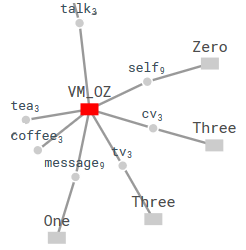
\includegraphics[width=.91\linewidth]{./images/transformational_semantics_of_oz/vm_OZ.png}}
  \caption{Stargazer visualization.}
\end{subfigure}
\caption{Transforming VM into \picalc{} process VM\_OZ\_PI.}
\label{tra_vm_OZ}
\end{figure}

\lstinputlisting[backgroundcolor=\color{white},caption={ the process VM\_OZ\_PI in ABC code.},captionpos=b, label={tra_vm_OZ_listing}]{listings/vm_OZ.abc}